En este capítulo se dispone el análisis realizado en base a los requisitos
presentados en el capítulo~\ref{chap:requisitos}, haciendo uso del lenguaje de
modelado UML. Concretamente, el capítulo describe:

\begin{itemize}
\item El \textbf{modelo conceptual} de los datos usados en la aplicación,
  elaborado a partir de los requisitos de información.
\item Los \textbf{casos de uso}, que describen los pasos que componen los
  procesos habituales del proyecto.
\item El \textbf{modelo de comportamiento} del sistema, donde se identifican las
  operaciones que se llevarán a cabo.
\item El \textbf{modelo de interfaz de usuario}, en el que se presenta un
  prototipo de la navegación y de las interfaces.
\end{itemize}

\section{Modelo conceptual}

De acuerdo a lo reflejado en el apartado~\ref{sec:requisitos-informacion} se
presenta el diagrama~\ref{fig:modelo-conceptual} en el que se identifican los
principales tipos de datos, sus atributos y las relaciones entre ellos.

\begin{figure}[hp]
  \centering
  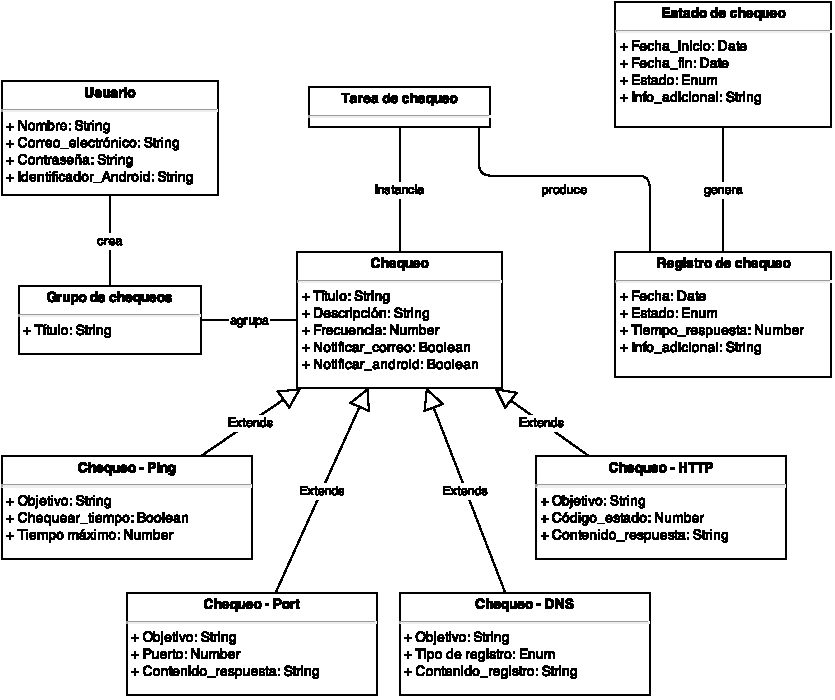
\includegraphics[width=\textwidth]{4_analisis/diagrama_clases_conceptuales}
  \caption{Modelo conceptual}
  \label{fig:modelo-conceptual}
\end{figure}

A continuación se detallan cada uno de los tipos de datos reflejados en el
modelo conceptual.

\subsection{Usuario}

Representa a un usuario de la aplicación que tiene intención de dar de alta
chequeos.

\begin{description}
\item[Nombre] Nombre elegido por el usuario.
\item[Correo electrónico] Dirección de correo electrónico.
\item[Contraseña] Contraseña para el login del usuario.
\item[Identificador Android] Identificador único del dispositivo Android del usuario.
\end{description}

\textbf{Relaciones}
\begin{itemize}
\item Un \textbf{usuario} puede crear \textbf{grupos de chequeos}.
\end{itemize}

\subsection{Grupo de chequeos}

Representa a una agrupación de chequeos relacionados con los que operar de forma
conjunta.

\begin{description}
\item[Título] Título para identificar al grupo de chequeos.
\end{description}

\textbf{Relaciones}

\begin{itemize}
\item Un \textbf{grupo de chequeos} pertenece a un \textbf{usuario}.
\item Un \textbf{grupo de chequeos} agrupa un conjunto de \textbf{chequeos}.
\end{itemize}

\subsection{Chequeo}

Representa un chequeo o punto de vigilancia sobre un servicio remoto.

\begin{description}
\item[Título] Título para identificar al chequeo.
\item[Descripción] Información adicional en forma textual sobre el chequeo.
\item[Frecuencia de chequeo] Frecuencia temporal del chequeo, expresada en minutos.
\item[Notificar por correo] Indica si los cambios de estado del chequeo deben notificarse por correo electrónico.
\item[Notificar por Android] Indica si los cambios de estado del chequeo deben notificarse por la aplicación Android.
\end{description}

\textbf{Relaciones}

\begin{itemize}
\item Un \textbf{chequeo} pertenece a un \textbf{grupo}.
\item Un \textbf{chequeo} lanza periódicamente \textbf{tareas de chequeo}.
\item De la ejecución de un \textbf{chequeo} se generan \textbf{registros de chequeo}.
\item De los cambios de estado en un \textbf{chequeo} se generan \textbf{registros de estado de chequeo}.
\end{itemize}

\subsection{Registro de chequeo}

Representa el resultado de la ejecución de un chequeo en un momento dado.

\begin{description}
\item[Fecha] Fecha y hora en la que se obtuvo este registro.
\item[Estado] Resultado del lanzamiento del chequeo. El estado puede ser
  \textit{Up}, que indica que el objetivo está funcionando; \textit{Down}, que
  indica que el objetivo no está funcionando correctamente; y \textit{Error},
  que indica que hubo un problema lanzando el chequeo.
\item[Tiempo de respuesta] \textit{(solo para chequeos tipo Ping)} indica el
  tiempo de respuesta medio obtenido al lanzar el chequeo.
\item[Información adicional] Datos extra en caso de que el estado no sea \textit{Up}.
\end{description}

\textbf{Relaciones}

\begin{itemize}
\item Es generado por una \textbf{tarea de chequeo} y pertenece a un \textbf{chequeo}.
\item Puede dar lugar al registro de un \textbf{estado de chequeo}.
\end{itemize}


\subsection{Estado de chequeo}

Representa un cambio de estado de un chequeo, detectado tras analizar un registro de chequeo.

\begin{description}
\item[Fecha de inicio] La fecha y hora en la que el chequeo entró en este estado.
\item[Fecha de fin] La fecha y hora en la que el chequeo salió de este estado.
\item[Estado] Definición del estado del chequeo. El estado puede ser
  \textit{Up}, que indica que el objetivo está funcionando; \textit{Down}, que
  indica que el objetivo no está funcionando correctamente; y \textit{Error},
  que indica que hubo un problema lanzando el chequeo.
\item[Información adicional] Información adicional sobre el estado.
\end{description}

\textbf{Relaciones}

\begin{itemize}
\item Un \textbf{estado de chequeo} pertenece a un \textbf{chequeo}, y se genera cuando en un \textbf{registro de
    chequeo} y se detecta un cambio de estado.
\end{itemize}

\subsection{Chequeo - Ping}

Representa un chequeo mediante paquetes ICMP.

\begin{description}
\item[Objetivo] Identificador de la máquina a la que enviar el ping. Debe ser un
  \textit{hostname} o una IP.
\item[Chequear tiempo?] Indica si además de chequear que la máquina responde al
  ping, también se debe chequear que el tiempo de respuesta sea menor que el indicado.
\item[Tiempo máximo] Tiempo de respuesta máximo permitido.
\end{description}

\textbf{Relaciones}

\begin{itemize}
\item Extiende a un \textbf{chequeo}
\end{itemize}

\subsection{Chequeo - Port}

Representa un chequeo de un puerto en un servidor remoto.

\begin{description}
\item[Objetivo] Identificador de la máquina a chequear.
\item[Puerto objetivo] Puerto remoto en la máquina que se chequeará.
\item[Contenido de respuesta] \textit{(opcional)} Cadena de caracteres que
  deberá estar presente en la respuesta obtenida de la máquina remota.
\end{description}

\textbf{Relaciones}

\begin{itemize}
\item Extiende a un \textbf{chequeo}
\end{itemize}


\subsection{Chequeo - DNS}

Representa un chequeo de registros DNS sobre un dominio.

\begin{description}
\item[Objetivo] Dominio sobre el que realizar el chequeo de DNS.
\item[Tipo de registro] Tipo de registro DNS a verificar. Puede ser A, AAAA, CNAME, MX y TXT.
\item[Contenido de registro] El contenido que debe tener el registro a consultar.
\end{description}

\subsection{Chequeo - HTTP}

Representa un chequeo mediante peticiones HTTP sobre un host remoto.

\begin{description}
\item[Objetivo] URL a verificar.
\item[Código de estado] Código que debe devolver la petición a la URL indicada.
\item[Cadena de respuesta] \textit{(opcional)} Cadena que debe encontrarse en la
  respuesta obtenida.
\end{description}

\textbf{Relaciones}

\begin{itemize}
\item Extiende a un \textbf{chequeo}
\end{itemize}

\section{Modelo de casos de uso}

El modelo de casos de uso representa las interacciones entre los actores y el
sistema, desarrollado a partir de los requisitos descritos anteriormente.

\subsection{Actores}

En este apartado se describen los diversos roles que juegan los usuarios del
sistema. Se reflejan todos ellos en el diagrama \ref{fig:actores}.

\begin{figure}[h]
  \centering
  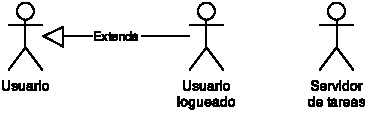
\includegraphics[width=0.7\textwidth]{4_analisis/diagrama_actores}
  \caption{Diagrama de actores}
  \label{fig:actores}
\end{figure}

\subsubsection{Usuario}

\begin{center}
  \begin{tabularx}{\textwidth}{|c|X|}
    \hline
     & Usuario \\

    \hline

    Descripción & Usuario libre de la aplicación, que puede haber hecho login previamente o no. \\

    \hline
  \end{tabularx}

\end{center}


\subsubsection{Usuario logueado}

\begin{center}
  \centering
  \begin{tabularx}{\textwidth}{|c|X|}
    \hline
     & Usuario logueado \\

    \hline

    Descripción & Usuario que previamente se ha registrado y ha hecho login en el sistema. \\

    \hline
  \end{tabularx}
\end{center}

\subsubsection{Servidor de tareas}

\begin{center}
  \centering
  \begin{tabularx}{\textwidth}{|c|X|}
    \hline
     & Servidor de tareas \\

    \hline

    Descripción & Servidor de tareas asíncronas que periódicamente lanza tareas que previamente se hayan dado de alta. \\

    \hline
  \end{tabularx}
\end{center}

\subsection{Subsistema de gestión de usuarios}

Los casos de uso pertenecientes a este subsistema pueden verse en la
figura~\ref{fig:subsistema-usuarios}

\begin{figure}[hp]
  \centering
  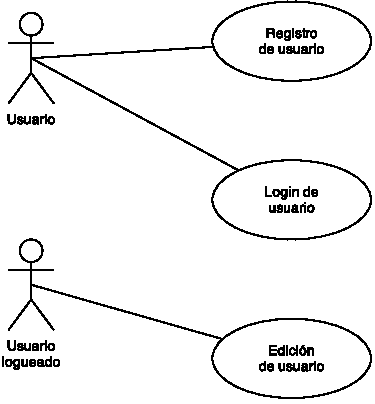
\includegraphics[width=0.5\textwidth]{4_analisis/diagrama_subsistema_gestion_usuarios}
  \caption{Casos de uso del subsistema de gestión de usuarios}
  \label{fig:subsistema-usuarios}
\end{figure}

\subsubsection{Caso de uso: registro de usuario}

\begin{description}
\item[Descripción] Un usuario no logueado se registra en la aplicación para poder dar de alta chequeos.
\item[Actores] \textit{Usuario}.
\item[Escenario principal] $\quad$
  \begin{enumerate}
  \item Un usuario decide registrarse en el sistema y accede al panel de registro.
  \item El \textit{usuario} introduce su nombre de usuario, dirección de correo electrónico y contraseña.
  \item El \textit{sistema} comprueba que los datos introducidos son correctos.
  \item El \textit{sistema} registra al usuario.
  \end{enumerate}
\item[Flujo alternativo] $\quad$
  \begin{description}
  \item[3a] Alguno de los datos introducidos es incompleto o no es correcto. El
    sistema informa al usuario del error.
  \item[3b] El nombre de usuario o dirección de correo electrónico ya han sido
    usados por otro usuario previamente. El sistema informa al usuario del error.
  \end{description}
\end{description}

\subsubsection{Caso de uso: login de usuario}


\begin{description}
\item[Descripción] Un usuario no logueado pero previamente registrado quiere hacer login en la aplicación.
\item[Actores] \textit{Usuario}.
\item[Escenario principal] $\quad$
  \begin{enumerate}
  \item Un usuario decide hacer login en el sistema.
  \item El \textit{usuario} accede al panel de login e introduce su nombre de usuario y contraseña.
  \item El \textit{sistema} comprueba que los datos introducidos son correctos.
  \item El \textit{sistema} loguea al usuario
  \end{enumerate}
\item[Flujo alternativo] $\quad$
  \begin{description}
  \item[3a] Alguno de los datos introducidos no tiene el formato correcto o está
    en blanco. El sistema informa al usuario del error.
  \item[3b] Los datos introducidos no corresponden a ningún usuario
    registrado. El sistema informa al usuario del error.
  \end{description}
\end{description}

\subsubsection{Caso de uso: edición de usuario}

\begin{description}
\item[Descripción] Un usuario logueado decide editar alguno de sus datos personales.
\item[Actores] \textit{Usuario logueado}.
\item[Escenario principal] $\quad$
  \begin{enumerate}
  \item El \textit{usuario} accede a su perfil de usuario a través del enlace \textit{Your profile}.
  \item El \textit{sistema} muestra los datos actuales.
  \item El \textit{usuario} edita los datos que quiera y envía el formulario.
  \item El \textit{sistema} comprueba los nuevos datos y guarda los cambios.
  \end{enumerate}
\item[Flujo alternativo] $\quad$
  \begin{description}
  \item[3a] Alguno de los nuevos datos no son válidos. El sistema informa del error al usuario.
  \end{description}
\end{description}

\subsection{Subsistema de gestión de grupos de chequeos}

Los casos de uso pertenecientes a este subsistema pueden verse en la figura~\ref{fig:subsistema-grupos}

\begin{figure}[hp]
  \centering
  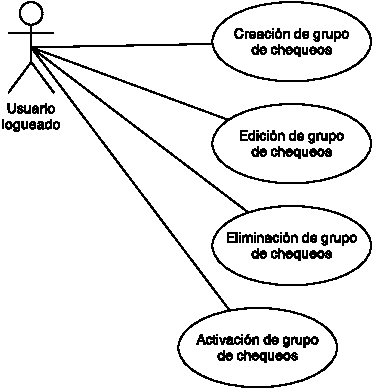
\includegraphics[width=0.6\textwidth]{4_analisis/diagrama_subsistema_gestion_grupos}
  \caption{Casos de uso del subsistema de gestión de grupos de chequeos}
  \label{fig:subsistema-grupos}
\end{figure}

\subsubsection{Caso de uso: creación de grupo de chequeos}

\begin{description}
\item[Descripción] Un usuario logueado decide crear un grupo de chequeos.
\item[Actores] \textit{Usuario logueado}.
\item[Escenario principal] $\quad$
  \begin{enumerate}
  \item El \textit{usuario} decide crear un nuevo grupo de chequeos.
  \item El \textit{usuario} pulsa en el botón de \textit{Añadir grupo}.
  \item El \textit{sistema} muestra el formulario para añadir nuevo grupo.
  \item El \textit{usuario} escribre el título del grupo.
  \item El \textit{sistema} valida el título introducido.
  \item El \textit{sistema} crea el nuevo grupo.
  \end{enumerate}
\item[Flujo alternativo] $\quad$

  \begin{description}
  \item[5a] El título introducido está en blanco o es inválido. El sistema
    informa al usuario del error.
  \end{description}
\end{description}


\subsubsection{Caso de uso: edición de grupo de chequeos}

\begin{description}
\item[Descripción] Un usuario logueado decide editar un grupo de chequeos.
\item[Actores] \textit{Usuario logueado}.
\item[Escenario principal] $\quad$
  \begin{enumerate}
  \item El \textit{usuario} decide editar un nuevo grupo de chequeos.
  \item El \textit{usuario} pulsa en el botón de \textit{Editar grupo} del grupo que quiera editar..
  \item El \textit{sistema} muestra el formulario para editar el grupo.
  \item El \textit{usuario} modifica el título del grupo.
  \item El \textit{sistema} valida el título introducido.
  \item El \textit{sistema} actualiza los datos del grupo.
  \end{enumerate}
\item[Flujo alternativo] $\quad$

  \begin{description}
  \item[5a] El título introducido está en blanco o es inválido. El sistema
    informa al usuario del error.
  \end{description}
\end{description}


\subsubsection{Caso de uso: eliminación de grupo de chequeos}

\begin{description}
\item[Descripción] Un usuario logueado decide eliminar un grupo de chequeos.
\item[Actores] \textit{Usuario logueado}.
\item[Escenario principal] $\quad$
  \begin{enumerate}
  \item El \textit{usuario} decide eliminar uno de sus grupos de chequeos.
  \item El \textit{usuario} pulsa en el botón de eliminar grupo.
  \item El \textit{sistema} muestra el formulario para confirmar la eliminación.
  \item El \textit{usuario} confirma la eliminación.
  \item El \textit{sistema} elimina los chequeos asociados al grupo.
  \item El \textit{sistema} elimina el grupo de chequeos.
  \end{enumerate}
\item[Flujo alternativo] $\quad$
  \begin{description}
  \item[3a] El \textit{usuario} no confirma la eliminación. El \textit{sistema}
    muestra la pantalla inicial.
  \end{description}
\end{description}

\subsubsection{Caso de uso: activación de grupo de chequeos}

\begin{description}
\item[Descripción] Un usuario logueado decide activar un grupo de chequeos.
\item[Actores] \textit{Usuario logueado}
\item[Escenario principal] $\quad$
  \begin{enumerate}
  \item El \textit{usuario} decide activar un grupo de chequeos.
  \item El \textit{usuario} pulsa en el botón de \textit{Activar grupo}.
  \item El \textit{sistema} itera por todos los chequeos pertenecientes al
    grupo, activando cada uno de ellos.
  \item El \textit{sistema} informa al usuario de que todos los chequeos han
    sido activados.
  \end{enumerate}

\item[Flujo alternativo] $\quad$
  \begin{description}
  \item[3a] El grupo no cuenta con chequeos. El \textit{sistema} no activa
    ningún chequeo.
  \end{description}
\end{description}

\subsection{Subsistema de gestión de chequeos}

Los casos pertenecientes a este subsistema pueden verse en la figura~\ref{fig:subsistema-chequeos}.

\begin{figure}[htbp]
  \centering
  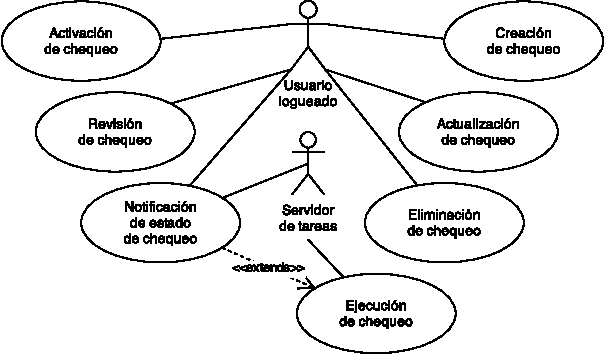
\includegraphics[width=\textwidth]{4_analisis/diagrama_subsistema_gestion_chequeos}
  \caption{Casos de uso del subsistema de gestión de chequeos}
  \label{fig:subsistema-chequeos}
\end{figure}

\subsubsection{Caso de uso: creación de chequeo}

\begin{description}
\item[Descripción] Un usuario logueado decide crear un chequeo dentro de un grupo.
\item[Actores] \textit{Usuario logueado}
\item[Escenario principal] $\quad$
  \begin{enumerate}
  \item El \textit{usuario} decide crear un chequeo dentro de un grupo de chequeos.
  \item El \textit{usuario} pulsa el botón de \textit{Añadir chequeo} de un grupo.
  \item El \textit{sistema} muestra el formulario de elección del tipo de chequeo.
  \item El \textit{usuario} elige el tipo de chequeo a añadir.
  \item El \textit{sistema} muestra el formulario con los campos según el tipo de chequeo elegido.
  \item El \textit{usuario} introduce los detalles del chequeo y envía el formulario.
  \item El \textit{sistema} recibe y comprueba que los datos son correctos.
  \item El \textit{sistema} da de alta el nuevo chequeo.
  \end{enumerate}
\item[Flujo alternativo] $\quad$
  \begin{description}
  \item[7a] Alguno de los datos introducidos no es correcto. El \textit{sistema}
    informa del error al usuario y muestra el formulario de nuevo.
  \end{description}
\end{description}


\subsubsection{Caso de uso: actualización de chequeo}

\begin{description}
\item[Descripción] Un usuario logueado decide editar un chequeo previamente creado..
\item[Actores] \textit{Usuario logueado}
\item[Escenario principal] $\quad$
  \begin{enumerate}
  \item El \textit{usuario} decide editar un chequeo dentro de un grupo de chequeos.
  \item El \textit{usuario} pulsa el botón de \textit{Editar chequeo}.
  \item El \textit{sistema} muestra el formulario con los campos rellenos con la información del chequeo elegido..
  \item El \textit{usuario} modifica los detalles del chequeo y envía el formulario.
  \item El \textit{sistema} recibe y comprueba que los datos son correctos.
  \item El \textit{sistema} actualiza el chequeo.
  \end{enumerate}
\item[Flujo alternativo] $\quad$
  \begin{description}
  \item[5a] Alguno de los datos introducidos no es correcto. El \textit{sistema}
    informa del error al usuario y muestra el formulario de nuevo.
  \end{description}
\end{description}

\subsubsection{Caso de uso: eliminación de chequeo}

\begin{description}
\item[Descripción] Un usuario logueado decide eliminar un chequeo previamente creado..
\item[Actores] \textit{Usuario logueado}
\item[Escenario principal] $\quad$
  \begin{enumerate}
  \item El \textit{usuario} decide eliminar un chequeo dentro de un grupo de chequeos.
  \item El \textit{usuario} pulsa el botón de \textit{Eliminar chequeo}.
  \item El \textit{sistema} muestra el formulario de confirmación de eliminación
  \item El \textit{usuario} confirma la eliminación del chequeo.
  \item El \textit{sistema} elimina el chequeo.
  \end{enumerate}
\item[Flujo alternativo] $\quad$
  \begin{description}
  \item[4a] El \textit{usuario} no confirma la eliminación del chequeo. El
    \textit{sistema} vuelve a la pantalla inicial.
  \end{description}
\end{description}

\subsubsection{Caso de uso: activación de chequeo}

\begin{description}
\item[Descripción] Un usuario logueado decide activar un chequeo.
\item[Actores] \textit{Usuario logueado}
\item[Escenario principal] $\quad$
  \begin{enumerate}
  \item El \textit{usuario} decide activar un chequeo dentro de un grupo de chequeos.
  \item El \textit{usuario} pulsa el botón de \textit{activar chequeo}.
  \item El \textit{sistema} activa el chequeo.
  \end{enumerate}
\end{description}

\subsubsection{Caso de uso: ejecución de chequeo}

\begin{description}
\item[Descripción] El servidor de tareas tiene que lanzar un chequeo periódico.
\item[Actores] \textit{Servidor de tareas}
\item[Escenario principal] $\quad$
  \begin{enumerate}
  \item El \textit{servidor de tareas} pide los chequeos activos.
  \item El \textit{sistema} devuelve los chequeos activos.
  \item El \textit{servidor de tareas} elige un chequeo activo.
  \item El \textit{servidor de tareas} ejecuta el chequeo.
  \item El \textit{sistema} devuelve el resultado del chequeo.
  \item El \textit{servidor de tareas} comprueba el resultado del chequeo,
    guardándolo en la base de datos y, si difere del estado anterior del
    chequeo, lanzando el \textit{Caso de uso: notificación de estado de chequeo}.
  \end{enumerate}
\item[Flujo alternativo] $\quad$
  \begin{description}
  \item[2a] No hay chequeos activos. El \textit{sistema} devuelve una lista
    vacía. El \textit{servidor de tareas} permanece en reposo.
  \end{description}
\end{description}

\subsubsection{Caso de uso: noitificación de estado de chequeo}

\begin{description}
\item[Descripción] El servidor de tareas detecta un cambio de estado y lanza notificación.
\item[Actores] \textit{Servidor de tareas}
\item[Escenario principal] $\quad$
  \begin{enumerate}
  \item El \textit{servidor de tareas} detecta un cambio de estado de un chequeo.
  \item El \textit{servidor de tareas} comprueba el campo
    \textit{Notificar\_correo} del chequeo.
  \item El \textit{servidor de tareas} lanza una notificación por correo electrónico.
  \item El \textit{sistema} envía la notificación al usuario dueño del chequeo.

  \item El \textit{servidor de tareas} comprueba el campo
    \textit{Notificar\_android} del chequeo.
  \item El \textit{servidor de tareas} lanza una notificación Android.
  \item El \textit{sistema} envía la notificación al usuario dueño del chequeo.

  \end{enumerate}
\item[Flujo alternativo] $\quad$
  \begin{description}
  \item[2a] El chequeo no tiene activa la opción \textit{Notificar\_correo}. El
    \textit{servidor de tareas} no envía la notificación por correo.
  \item[5a] El chequeo no tiene activa la opción \textit{Notificar\_android}. El
    \textit{servidor de tareas} no envía la notificación por Android.
  \item[5b] El usuario no tiene dispositivo Android dado de alta. El
    \textit{servidor de tareas} no envía la notificación por Android.
  \end{description}
\end{description}

\section{Modelo de comportamiento}

Basándonos en los casos de uso anteriores se crea el modelo de comportamiento,
compuesto de diagramas de secuencia, en los que se identificarán las operaciones
del sistema, y de lo contratos de estas operaciones.

{\Huge TO-DO }



\section{Modelo de interfaz de usuario}

En esta sección se presenta una aproximación de la navegación y apariencia de la
interfaz de usuario, tanto de la plataforma web como de la aplicación móvil.

\subsection{Modelo de navegación}

El modelo de navegación de la aplicación web se presenta en la
figura~\ref{fig:modelo-navegacion-web}. El modelo de navegación de la aplicación
Android se presenta en la figura~\ref{fig:modelo-navegacion-android}

\begin{figure}[hbtp]
  \centering
  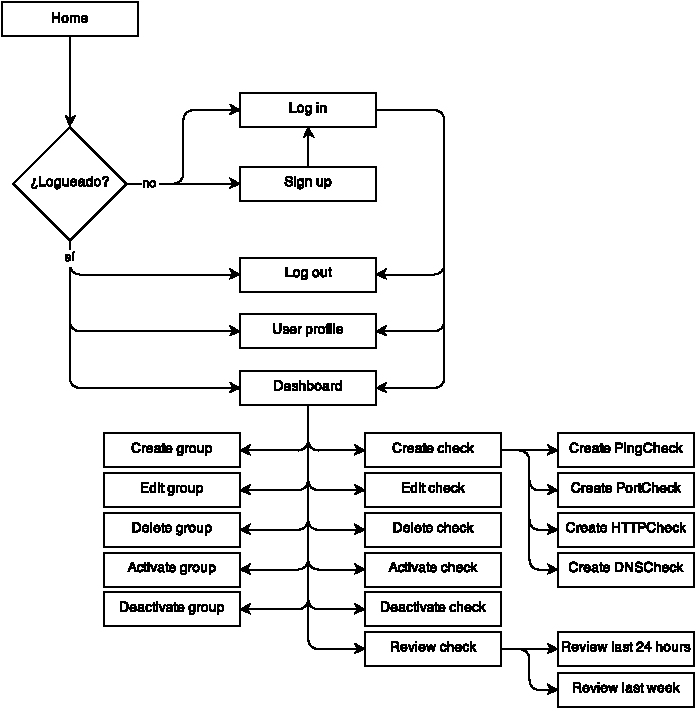
\includegraphics[width=0.8\textwidth]{4_analisis/diagrama_navegacion}
  \caption{Modelo de navegación de la aplicación web}
  \label{fig:modelo-navegacion-web}
\end{figure}

\begin{figure}[hbtp]
  \centering
  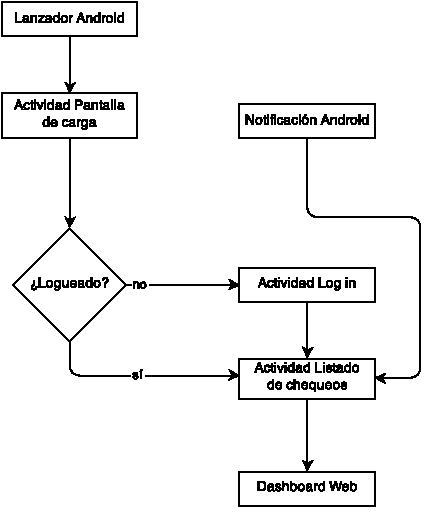
\includegraphics[width=0.6\textwidth]{4_analisis/diagrama_navegacion_android}
  \caption{Modelo de navegación de la aplicación Android}
  \label{fig:modelo-navegacion-android}
\end{figure}

\subsection{Prototipos visuales de la interfaz web}

A continuación se presentan los prototipos de las pantallas de la aplicación
web. En concreto:

\begin{itemize}
\item La figura \ref{fig:phome} representa la pantalla de bienvenida.
\item La figura \ref{fig:plogin} representa la pantalla con el formulario para
  iniciar sesión.
\item La figura \ref{fig:ppassword} representa la pantalla para recuperar la contraseña.
\item La figura \ref{fig:pregister} representa la pantalla para crear una cuenta de usuario.
\item La figura \ref{fig:pdashboard} representa la pantalla de dashboard, en la que se ve la lista de chequeos.
\item La figura \ref{fig:pdetail} representa la pantalla de detalle de chequeo.
\item La figura \ref{fig:pnewgroup} representa la pantalla de creación de nuevo grupo de chequeos.
\item La figura \ref{fig:pnewcheck} representa la pantalla de creación de nuevo chequeo.
\end{itemize}

\subsection{Prototipos visuales de la aplicación móvil}

Seguidamente se presentan los prototipos de las interfaces visuales de la
aplicación móvil. En particular:

\begin{itemize}
\item La figura \ref{fig:aloading} representa la pantalla de carga de la aplicación Android.
\item La figura \ref{fig:alogin} representa la pantalla de login.
\item La figura \ref{fig:alist} representa la pantalla de lista de chequeos.
\item La figura \ref{fig:anotify} representa una notificación recibida en el dispositivo.
\end{itemize}


\begin{figure}[htbp]
  \centering
  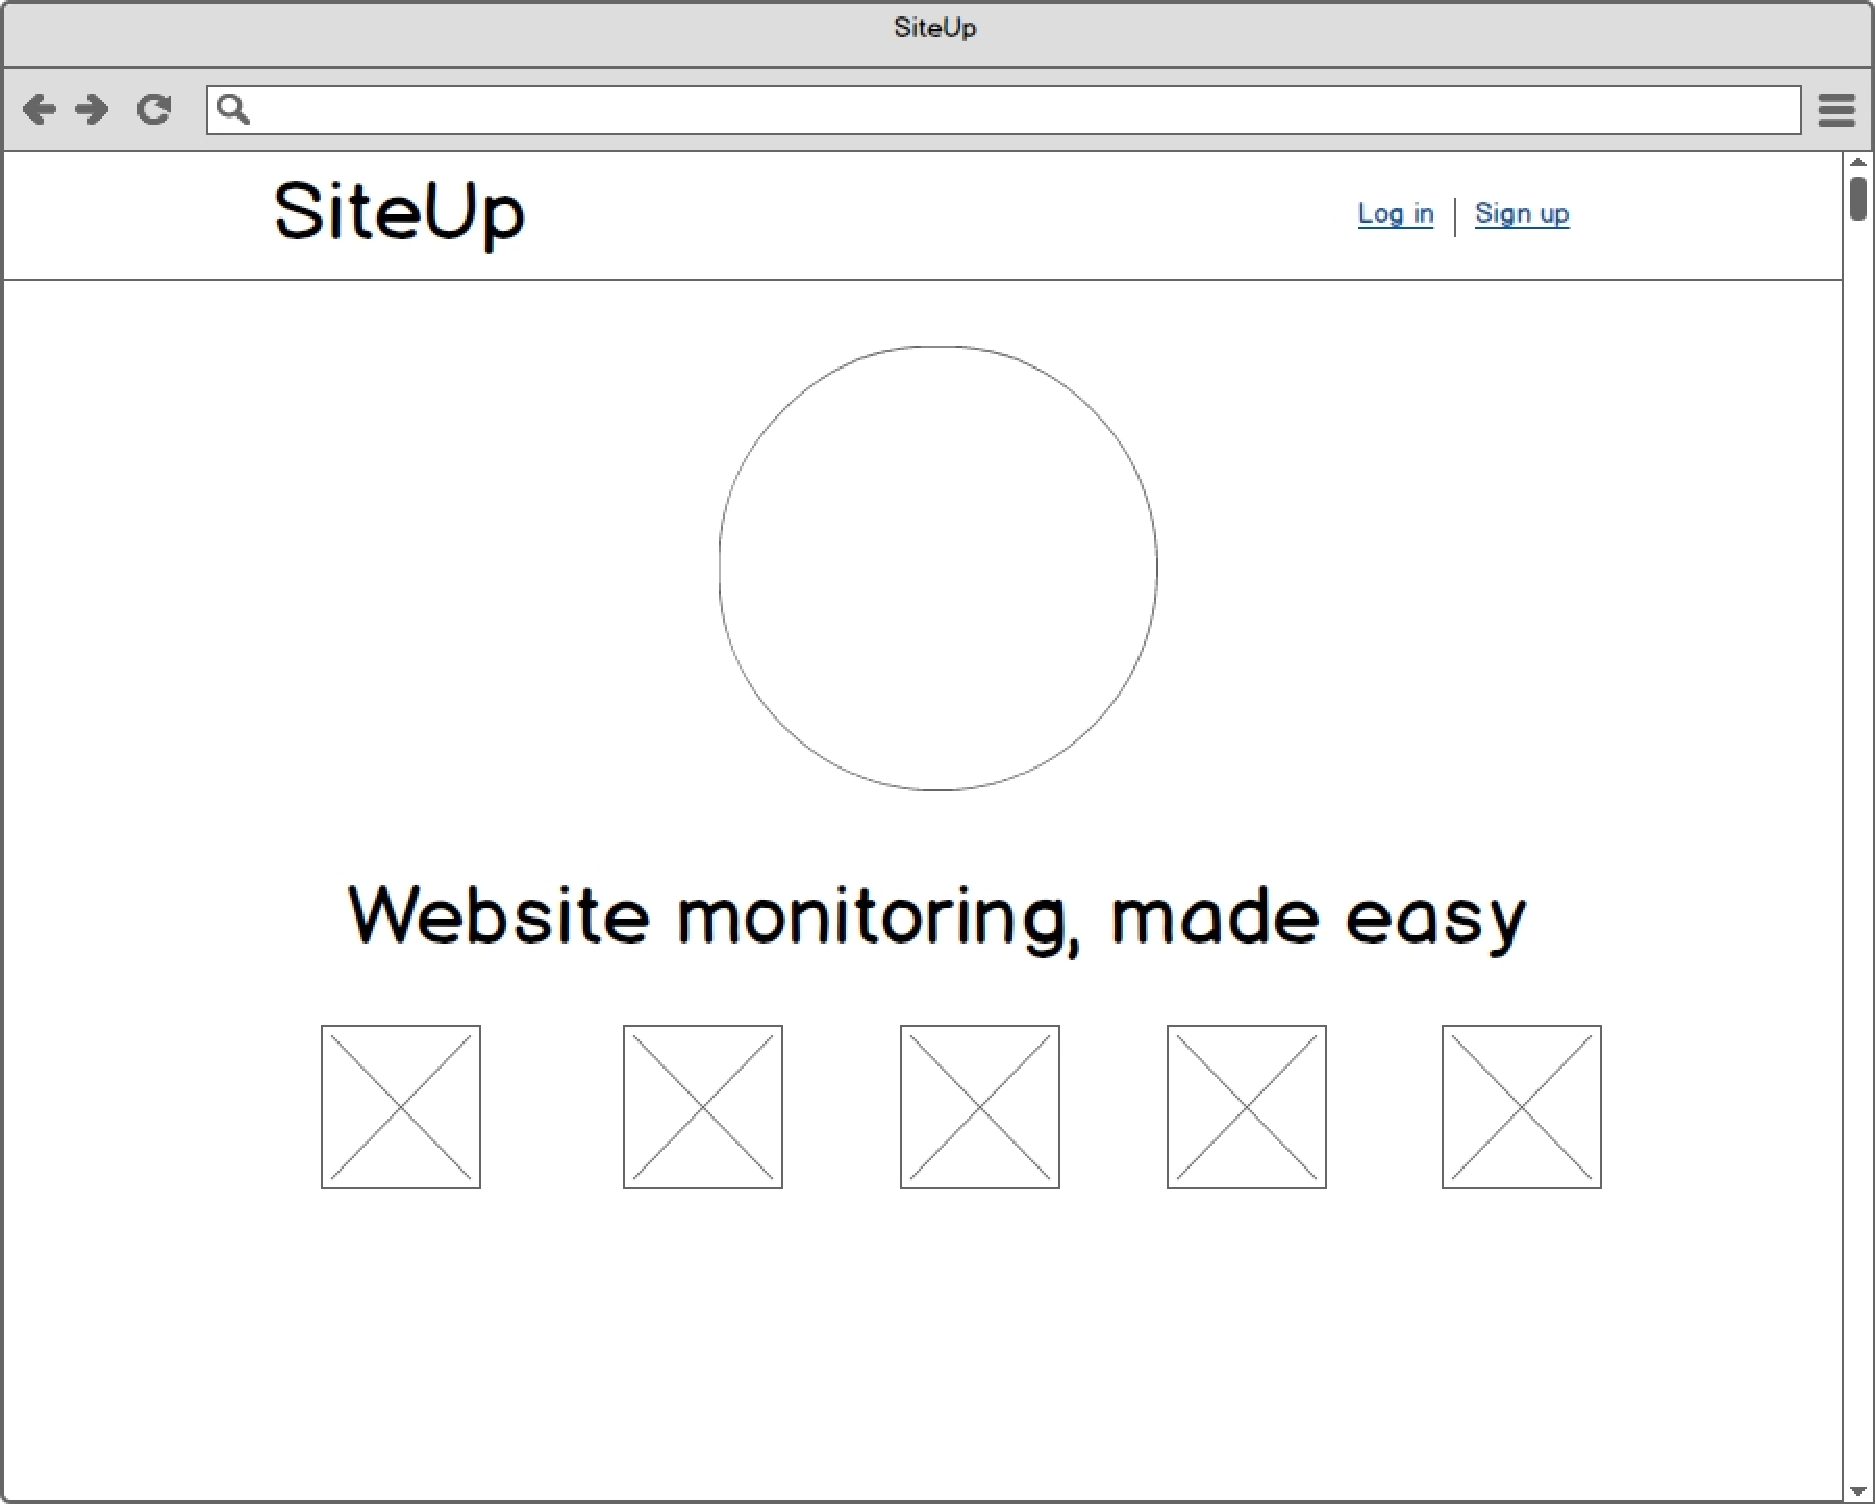
\includegraphics[width=0.8\textwidth, page=1]{4_analisis/pantallas}
  \caption{Home}
  \label{fig:phome}
\end{figure}

\begin{figure}[htbp]
  \centering
  \includegraphics[width=0.8\textwidth, page=2]{4_analisis/pantallas}
  \caption{Login}
  \label{fig:plogin}
\end{figure}

\begin{figure}[htbp]
  \centering
  \includegraphics[width=0.8\textwidth, page=3]{4_analisis/pantallas}
  \caption{Recuperación de contraseña}
  \label{fig:ppassword}
\end{figure}

\begin{figure}[htbp]
  \centering
  \includegraphics[width=0.8\textwidth, page=4]{4_analisis/pantallas}
  \caption{Registro de usuario}
  \label{fig:pregister}
\end{figure}

\begin{figure}[htbp]
  \centering
  \includegraphics[width=0.8\textwidth, page=5]{4_analisis/pantallas}
  \caption{Dashboard}
  \label{fig:pdashboard}
\end{figure}

\begin{figure}[htbp]
  \centering
  \includegraphics[width=0.8\textwidth, page=6]{4_analisis/pantallas}
  \caption{Detalle de chequeo}
  \label{fig:pdetail}
\end{figure}

\begin{figure}[htbp]
  \centering
  \includegraphics[width=0.8\textwidth, page=7]{4_analisis/pantallas}
  \caption{Creación de grupo de chequeos}
  \label{fig:pnewgroup}
\end{figure}


\begin{figure}[htbp]
  \centering
  \includegraphics[width=0.8\textwidth, page=8]{4_analisis/pantallas}
  \caption{Formulario genérico de creación de chequeo}
  \label{fig:pnewcheck}
\end{figure}



\begin{figure}[htbp]
  \centering
  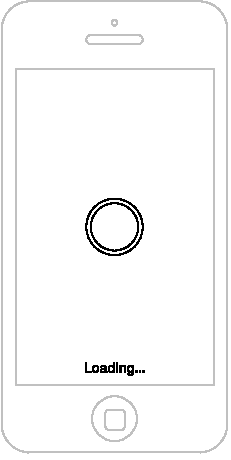
\includegraphics[width=0.3\textwidth]{4_analisis/android_loading}
  \caption{Pantalla de carga}
  \label{fig:aloading}
\end{figure}

\begin{figure}[htbp]
  \centering
  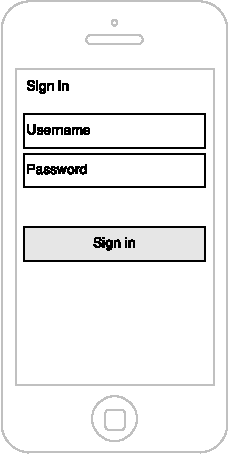
\includegraphics[width=0.3\textwidth]{4_analisis/android_login}
  \caption{Pantalla de login}
  \label{fig:alogin}
\end{figure}

\begin{figure}[htbp]
  \centering
  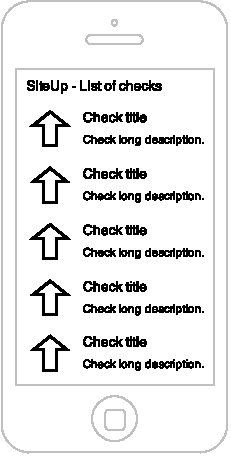
\includegraphics[width=0.3\textwidth]{4_analisis/android_list}
  \caption{Pantalla de listado de chequeos}
  \label{fig:alist}
\end{figure}

\begin{figure}[htbp]
  \centering
  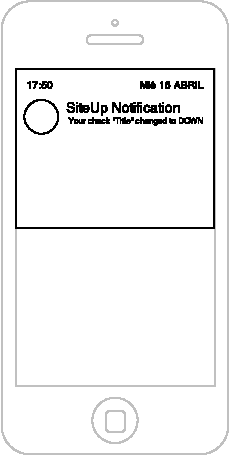
\includegraphics[width=0.3\textwidth]{4_analisis/android_notification}
  \caption{Pantalla de notificación}
  \label{fig:anotify}
\end{figure}


%%% Local Variables: 
%%% mode: latex
%%% TeX-master: "../memoria"
%%% End: 
